\section{Auswertung}

\subsection{Strahlenschutzmessung}

In Aufgabe 1 nahmen wir Messungen bezüglich des Strahlenschutzes vor. Dazu verwendeten wir ein mobiles Dosimeter und nahmen die aus Tabelle \ref{dft:Arbeitsplatz} bekannten Messdaten an verschiedenen Orten auf. Zur besseren Verdeutlichung, wo wir gemessen haben, folgt eine Skizze des Labors.

\vspace{5mm}

\begin{center}
    \minipanf    
        \makebox[\textwidth]{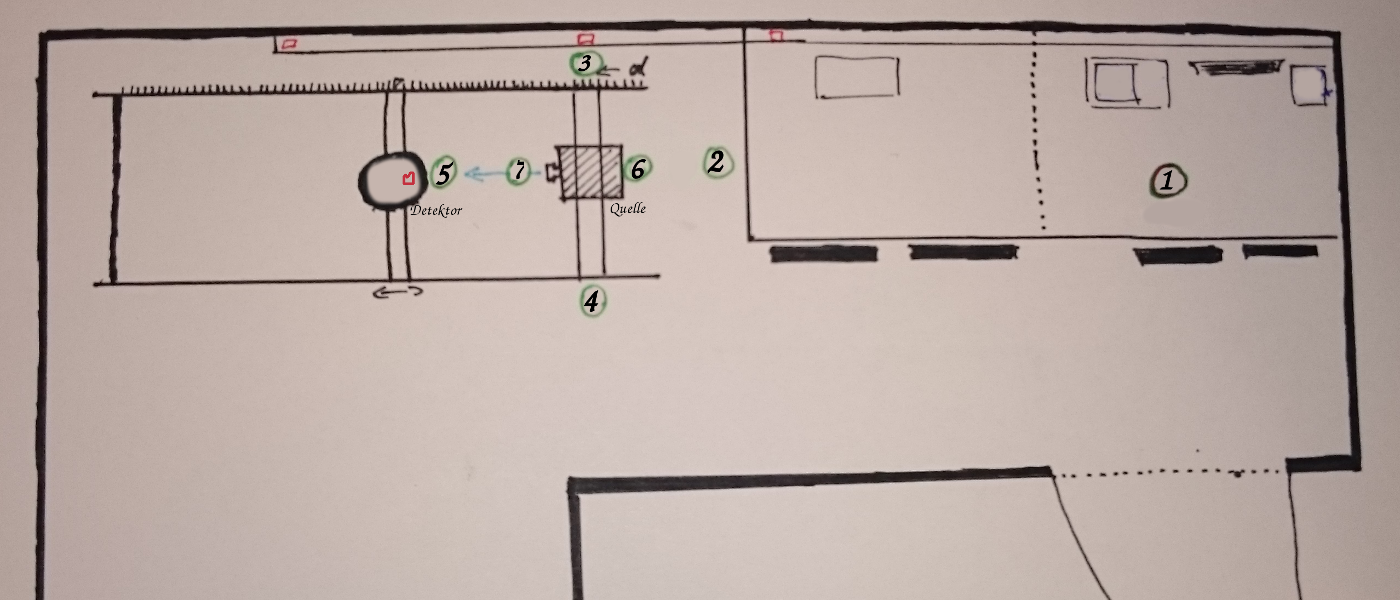
\includegraphics[width=1.4\linewidth, height=0.4\textheight]{pic/skizze}}
        \captionof{figure}{Raumskizze zu Messorten (nicht maßstabsgerecht)\\ 
                            \textbf{1:} Arbeitsplatz, \textbf{2:} 50cm hinter Quelle, \textbf{3:} 50cm rechts der Quelle, \textbf{4:} 50cm links, \textbf{5:} 50cm davor, \textbf{6:} 8cm dahinter, \textbf{7:} 8cm davor}
        \label{fig:skizze}
    \minipend
\end{center}

\vspace{5mm}

Die roten Kästchen im Bild bezeichnen die vier Punkte, an denen die BeO-Detektoren lagen. Die oberen drei liegen auf einer Steckerleiste, ca. 40cm unterhalb der Quelle. Das Kästchen bei \textbf{5} bezeichnet den \textquotedblleft Mitfahrer \textquotedblright.

\subsubsection{Strahlungswerte im Labor am Anfang des Versuchstages}
Zunächst gehen wir auf Tabelle \ref{dft:Arbeitsplatz} ein. Die Werte unterhalb des zweiten Trennstriches sind bei 
geöffnetem Kollimatorverschluss aufgenommen worden, während die darüber bei geschlossenem Verschluss notiert wurden. 
Man sieht, dass bei geschlossenem Stopfen  am Arbeitsplatz für einen Praktikanten, der eine Maximalbelastung von 6mSv
 im Jahr erreichen darf, kaum eine Gefahr besteht, diesen Grenzwert an einem Tag zu überschreiten. Um die maximale 
 Tagesdosis zu erreichen, benötigte dieser ca. 12,5 Stunden. Solange darf ein Praktikant oder Lehrling gesetzlich aber 
nicht zur Arbeit gezwungen werden.\\
Nähert man sich der Quelle, kann man bei 50cm Abstand einen deutlichen Anstieg in der Strahlendosis erkennen, was sich 
auch deutlich an der Zeit widerspiegelt, die sich der Praktikant in dieser Nähe aufhalten sollte. Diese ist nun sechsmal
kleiner als am Arbeitsplatz.\\
Zu beachten sei auch, dass der Kollimator auf linker und rechter Seite offenbar weniger stark abschirmt. Dies ist ein 
interessantes Ergebnis, da sich die maximale Aufenthaltsdauer damit auch deutlich verkürzt 50cm vor der Quelle ist die
Abschirmung erwartungsgemäß am schwächsten, da dort der Kollimatorverschluss vorhanden ist und dieser nicht so gut abschirmen
kann wie die Standardwände. Dementsprechend logisch ist es, sich nicht längere Zeit in den Strahl zu stellen, was sich in 
einer Maximaldauer von $t_{max} \cong 17min$ zeigt. Dementsprechend fällt auch das Ergebnis der Messung 8cm vor der Quelle auf. 
Eine Aufenthaltsdauer unterhalb von 2min am Tag ist hier also angebracht.
Im Allgemeinen sollte man deshalb seinen Arbeitsplatz nicht neben der Messanordnung aufbauen, auch wenn es aus Bequemlichkeit 
zunächst sinnvoll erscheinen mag. Es verkürzt nicht nur die Laufwege, die man im Raum hat, sondern auch erhöht auch die Gefahr, 
an strahlenbedingten Leiden zu erkranken.

\subsubsection{Strahlendosis im Labor über 2 Tage}
Nun schauen wir uns Tabelle \ref{dft:Raum} an. Hier wurden Daten über fast zwei Tage gesammelt. Man sieht 
deutlich, dass der Mitfahrer, welcher am Versuchstag immer schwankenden Werten ausgesetzt war, eine Dosis von 
etwa 0,5mSv gemessen hat. Dies entspricht etwa der Hälfte von dem, was eine Standardperson in einem Jahr an 
künstlicher Strahlung erfahren darf. Fraglich ist allerdings, ob dieser Wert nicht ein Ergebnis von Störungen, 
die andere Experimente verursacht haben, ist.  